\chapter{Via Ferrata les Prises de la Bastille, Grenoble}

\section*{The basics}

\place{Grenoble} possess the only urban \emph{via ferrata} in France, \place{Les Prises de la Bastille}. It is an ideal spot for getting in shape and training for more inaccessible \emph{ferratas}. But don't get fooled, its level goes from difficult enough to very difficult, above the maximum quotation you find in high mountain at \place{\nameref{ch:via-ferrata-lacs-robert}}. Official information about the \emph{via} status can be found at \href{https://www.grenoble-montagne.com/2268-via-ferrata-de-la-bastille.htm}{Grenoble montagne website} (in French).

\section*{Getting there}

Joining the \emph{ferrata} is pretty straightforward and just 900~m from \place{Grenoble}'s train station. Figure~\ref*{fig:map-via-ferrata-les-prises-de-la-bastille} provides in red the access through the \place{Route de Lyon 22}, only 100~m from \place{Porte de France}. The full map can also be found in my \href{https://www.alltrails.com/fr/explore/map/carte-30-decembre-2022-ac9edbb}{All Trails} profile.

\begin{figure}[!ht]
\centering%
\includegraphics[width=\columnwidth, clip]{media/maps/via-ferrata-les-prises-de-la-bastille-detail}
\caption{\label{fig:map-via-ferrata-les-prises-de-la-bastille}Path to the \emph{via ferrata} from the train station (red), transition across the park from first to second segment (green), and final approach to last part (blue).}
\end{figure}

\begin{figure}[!ht]
	\centering%
	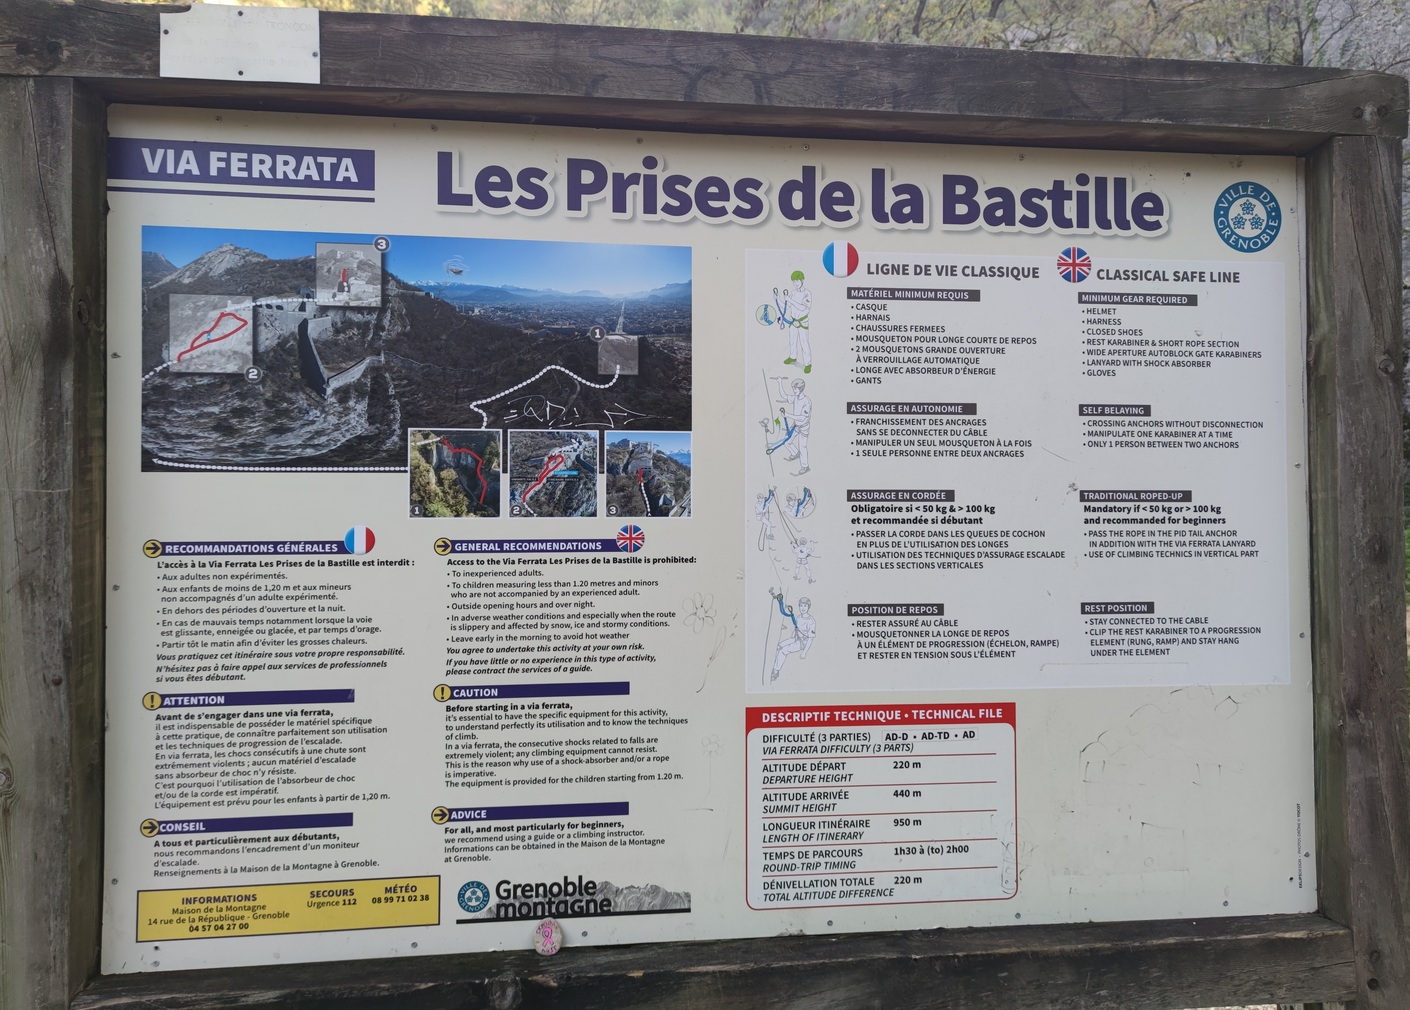
\includegraphics[width=\columnwidth, clip]{media/pictures/via-ferrata-les-prises-de-la-bastille-1}
	\caption{\label{fig:via-ferrata-les-prises-de-la-bastille-1}Panel indicating the start of \emph{via ferrata}.}
\end{figure}

\begin{figure}[!ht]
	\centering%
	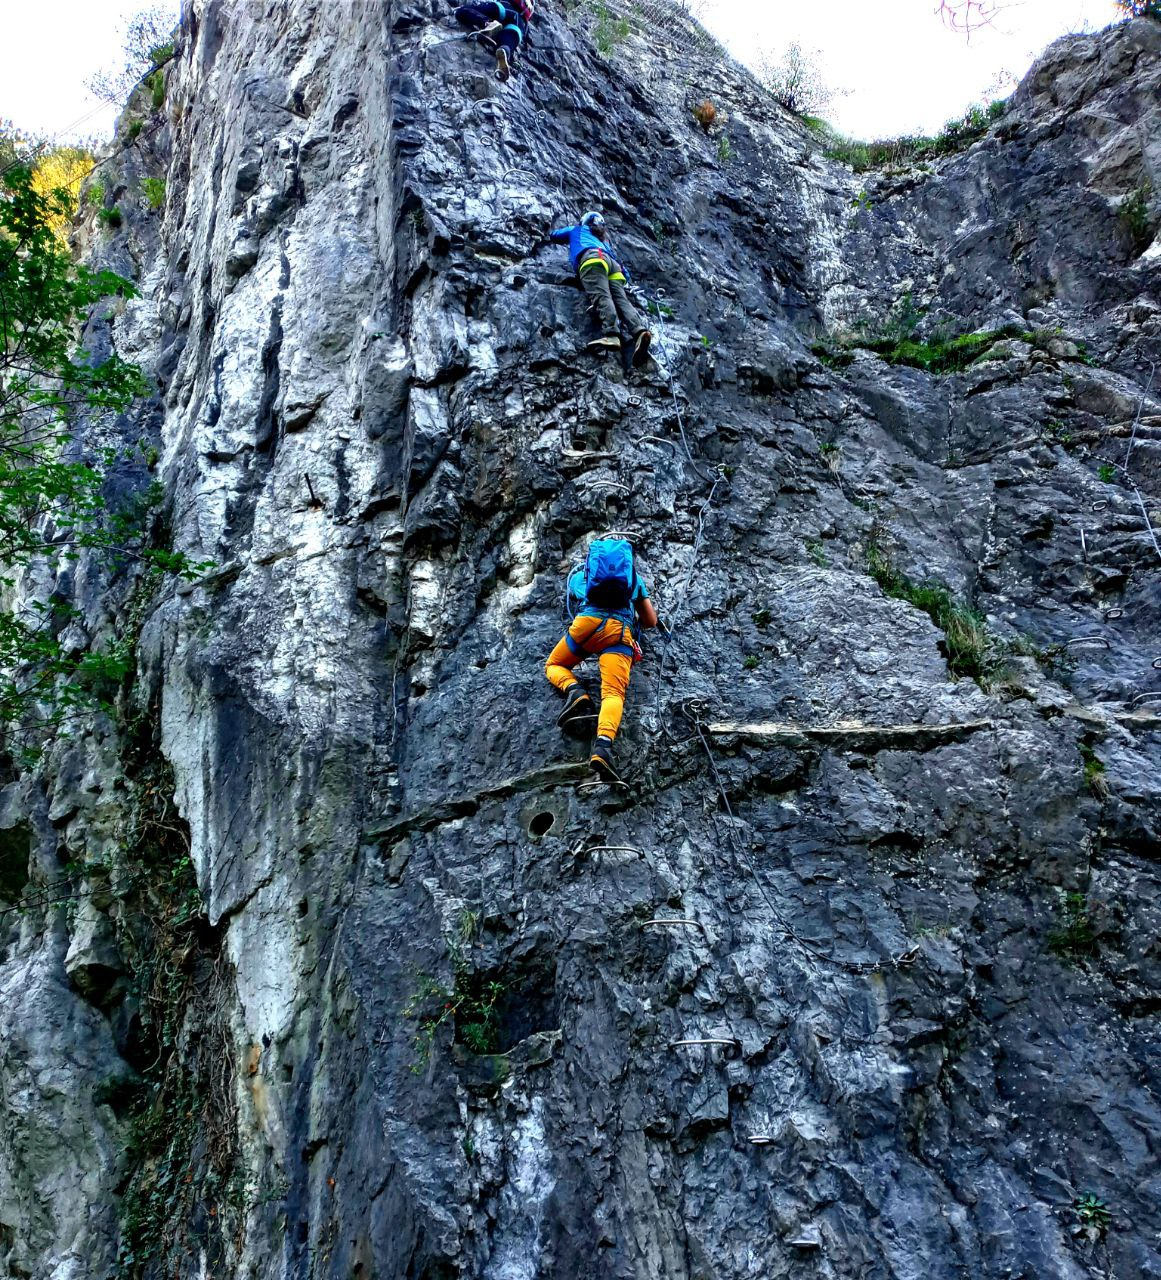
\includegraphics[width=\columnwidth, clip]{media/pictures/via-ferrata-les-prises-de-la-bastille-2}
	\caption{\label{fig:via-ferrata-les-prises-de-la-bastille-2}Panel indicating the start of \emph{via ferrata}.}
\end{figure}

\begin{figure}[!ht]
	\centering%
	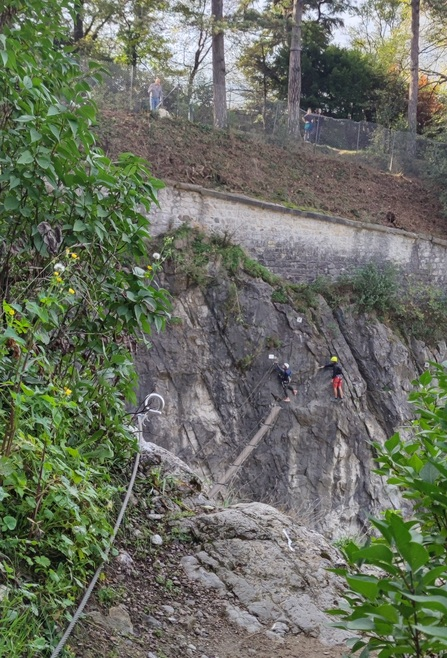
\includegraphics[width=\columnwidth, clip]{media/pictures/via-ferrata-les-prises-de-la-bastille-3}
	\caption{\label{fig:via-ferrata-les-prises-de-la-bastille-3}Panel indicating the start of \emph{via ferrata}.}
\end{figure}

\begin{figure}[!ht]
	\centering%
	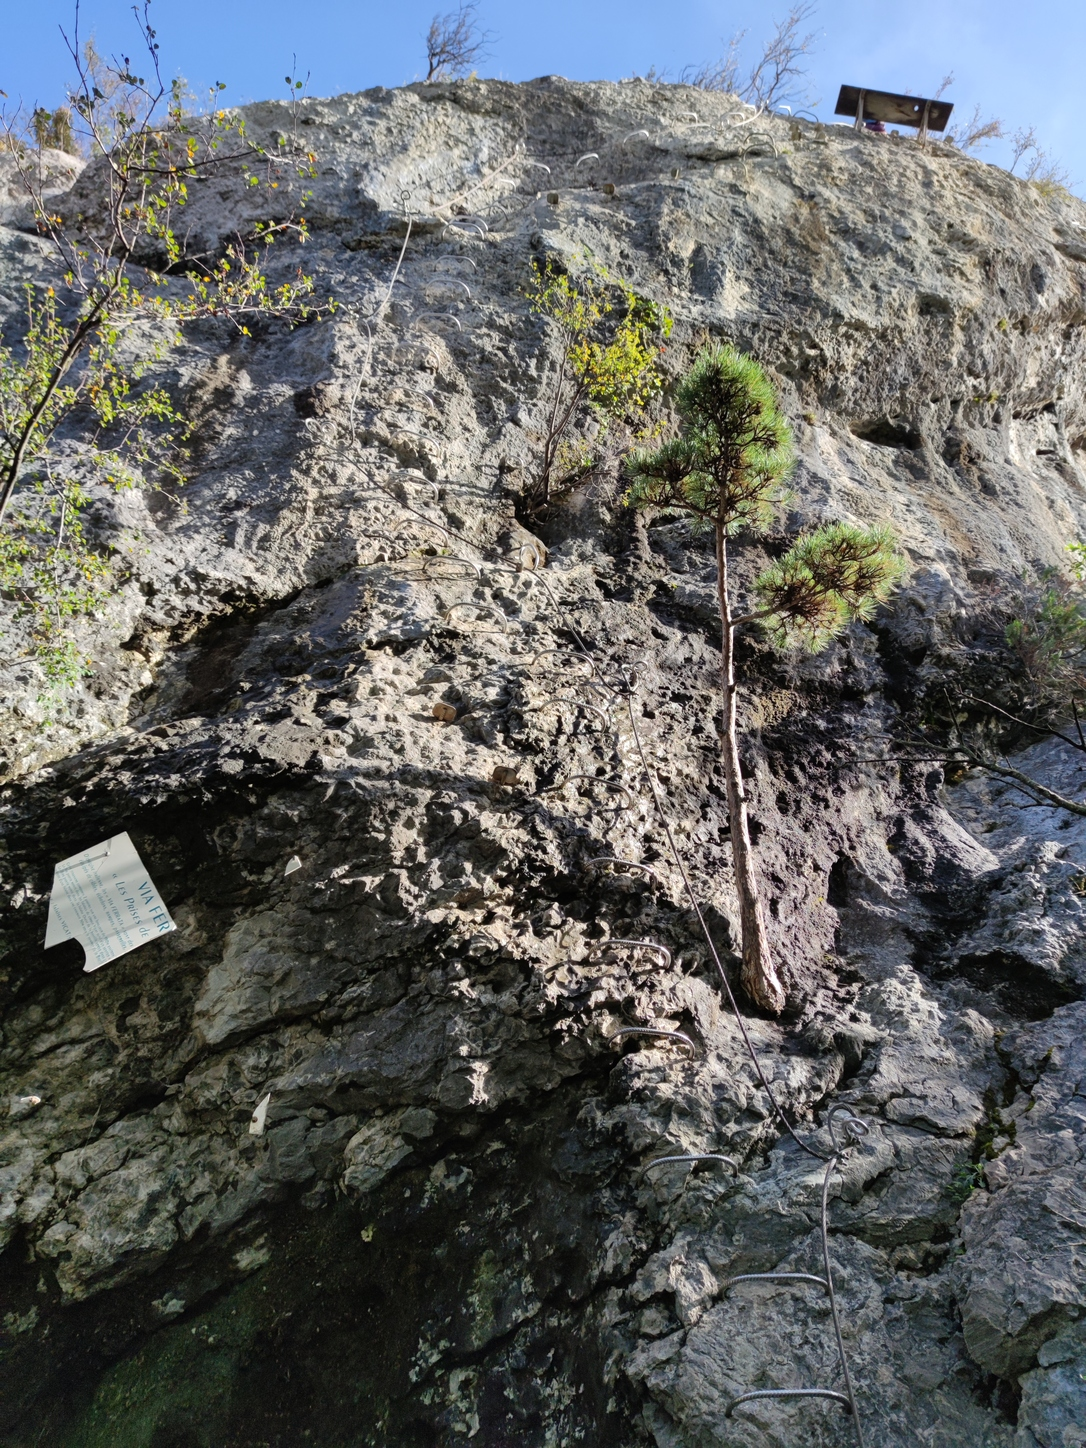
\includegraphics[width=\columnwidth, clip]{media/pictures/via-ferrata-les-prises-de-la-bastille-4}
	\caption{\label{fig:via-ferrata-les-prises-de-la-bastille-4}Panel indicating the start of \emph{via ferrata}.}
\end{figure}

\begin{figure}[!ht]
	\centering%
	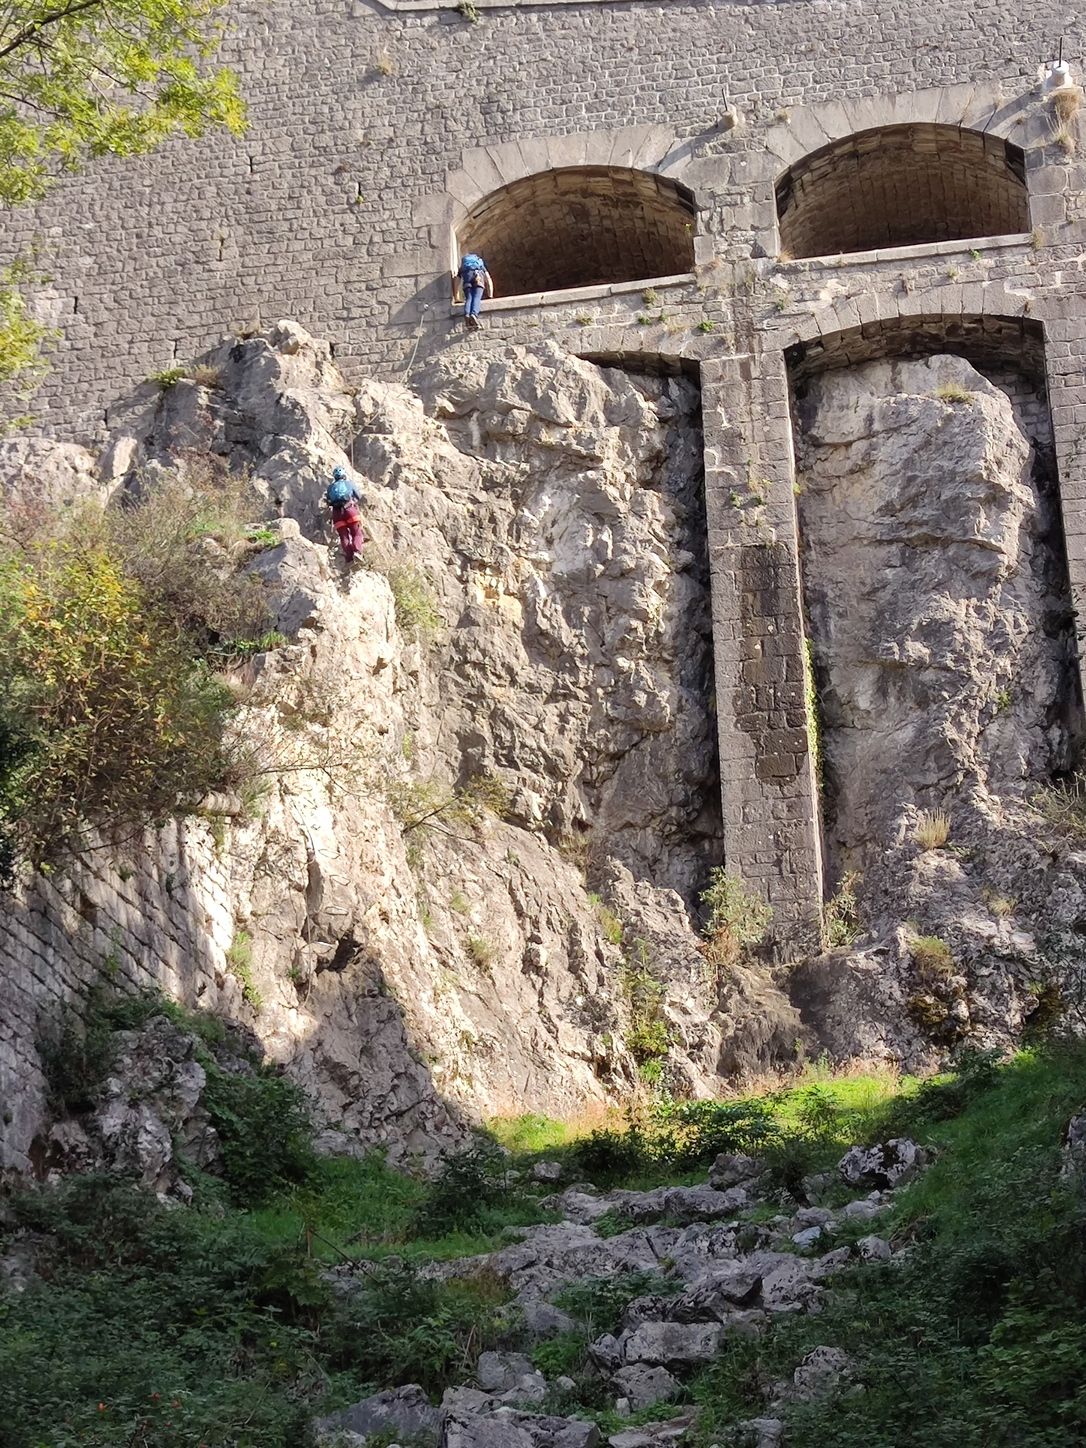
\includegraphics[width=\columnwidth, clip]{media/pictures/via-ferrata-les-prises-de-la-bastille-5}
	\caption{\label{fig:via-ferrata-les-prises-de-la-bastille-5}Panel indicating the start of \emph{via ferrata}.}
\end{figure}

\section*{The via ferrata}

\endinput